%%%%%%%%%%%%%%%%%%%%%%%%%%%%%%%%%%%%%%%%%
% FRI Data Science_report LaTeX Template
% Version 1.0 (28/1/2020)
% 
% Jure Demšar (jure.demsar@fri.uni-lj.si)
%
% Based on MicromouseSymp article template by:
% Mathias Legrand (legrand.mathias@gmail.com) 
% With extensive modifications by:
% Antonio Valente (antonio.luis.valente@gmail.com)
%
% License:
% CC BY-NC-SA 3.0 (http://creativecommons.org/licenses/by-nc-sa/3.0/)
%
%%%%%%%%%%%%%%%%%%%%%%%%%%%%%%%%%%%%%%%%%


%----------------------------------------------------------------------------------------
%	PACKAGES AND OTHER DOCUMENT CONFIGURATIONS
%----------------------------------------------------------------------------------------
\documentclass[fleqn,moreauthors,10pt]{ds_report}
\usepackage[english]{babel}

\graphicspath{{fig/}}




%----------------------------------------------------------------------------------------
%	ARTICLE INFORMATION
%----------------------------------------------------------------------------------------

% Header
\JournalInfo{FRI Natural language processing course 2021}

% Interim or final report
\Archive{Project report} 
%\Archive{Final report} 

% Article title
\PaperTitle{Qualitative Research on Discussions - text categorization} 

% Authors (student competitors) and their info
\Authors{Krištof Zupan, Gal Menaše, and Nejc Mušič}

% Advisors
\affiliation{\textit{Advisors: Slavko Žitnik}}

% Keywords
\Keywords{}
\newcommand{\keywordname}{Keywords}


%----------------------------------------------------------------------------------------
%	ABSTRACT
%----------------------------------------------------------------------------------------

\Abstract{This project investigates the potential of large language models (LLMs) to perform qualitative discourse analysis by categorizing textual data from online discussions. Initially, traditional methods such as TF-IDF and bag-of-words models were employed as baselines, using classifiers like XGBoost, Logistic Regression, Random Forest, and SVM. The performance of these models was moderate, with F1-micro scores ranging from 0.5492 to 0.6246. Subsequently, advanced models including BERT and its large variant were fine-tuned for this task, yielding improved results with validation and test F1-micro scores of 0.733 and 0.726 for the base BERT, and 0.75 and 0.698 for the large BERT, respectively. Additionally, GPT-3.5 was utilized with zero-shot and few-shot prompting, where the latter significantly boosted the F1-micro score to 0.636. This study demonstrates that with fine-tuning and appropriate prompting, LLMs can effectively categorize discussions, thus automating qualitative discourse analysis. Further research is suggested to enhance these methods, especially with larger and more diverse datasets.

}

%----------------------------------------------------------------------------------------

\begin{document}

% Makes all text pages the same height
\flushbottom 

% Print the title and abstract box
\maketitle 

% Removes page numbering from the first page
\thispagestyle{empty} 

%----------------------------------------------------------------------------------------
%	ARTICLE CONTENTS
%----------------------------------------------------------------------------------------

\section*{Introduction}
    
    Qualitative discourse analysis is a method used by social scientists for studying human interactions within textual data, involving understanding the underlying meanings, context, and perspectives expressed within conversations or written communication. Since this task is demanding for human "coders," we will replace them with the use of large language models. Our goal is to develop a highly reliable language model capable of categorizing postings in online discussions. We will be using a provided corpus, including an online discussion about the story "The Lady, or the Tiger?" Our aim is also to ensure that the model is capable of performing this task on other online discussions. 


    To achieve this, we came up with the following plan. Firstly, we will use traditional analysis techniques such as TF-IDF and bag-of-words models. These methods will serve as our baseline models, allowing us to establish a foundation for comparison.  Next, we'll move on to using more advanced models like BERT for sequence classification. Additionally, we'll fine-tune BERT for our task, tweaking its settings to improve how it categorizes online discussions. This way, we aim to make our language model better for analyzing conversations. We will also use gpt3.5-model with prompts to try to categorize text. We will try zero-shot and few-shot techniques. We will also gather explanations from model for result analysis.
    
    

\section*{Literature review}
    
    First we skimmed through James Paul Gee's book "An Introduction to Discourse Analysis: Theory and Method" \cite{gee2014introduction}. The book provides a fairly detailed description of the field of discourse analysis. We find chapters such as the seven building tasks of language, the distinction between situated meanings and discourse models, discourse analysis, and a detailed example of discourse analysis. However, we did not come across any practices or methods related to NLP. We will use it when encountering any unfamiliar definitions in the future. 
    
    In "ChatGPT in education: a discourse analysis of worries and concerns on social media" publication by Lingyao Li, Zihui Ma, Lizhou Fan, Sanggyu Lee, Huizi Yu, and Libby Hemphill \cite{li2305chatgpt} they performed sentiment classification with the use of RoBERTa transformer model on twitter discourse in order to get tweets with negative sentiment. On these tweets BERTopic model was used to get sentence embeddings in latent space. This latent space consists of high-dimensional vectors so to battle the "curse od dimensionality" UMAP (Uniform Manifold Approximation and Projection) dimensionality reduction method was used. After the k-means clustering algorithm was used on embeddings to extract topic information from similar embeddings. On tweets in the same cluster the Term Frequency-Inverse Document Frequency method (c-TF-IDF) was used to extract the topical keywords and representative tweets from each cluster for different topic categorization. 
    
    There was also "TopicGPT: A Prompt-based Topic Modeling Framework" article by Chau Minh Pham, Alexander Hoyle, Simeng Sun, and Mohit Iyyer \cite{pham2023topicgpt} that heavely relied on prompts to the TopicGPT model for topic categorization.This article gave us another promising idea. We will use prompts with definitions for categories to classify text.

    We also analyzed the work that was done in a paper from the university of Birmingham. "Assessing the potential of LLM-assisted annotation for corpus-based pragmatics and discourse analysis" \cite{llm2023analysis}, the paper focuses on using LLM GPT models to annotate and analyse discourse. In this paper the proposed methedology is using prompts to analyse text. The results of the paper shows that in the specific task the GPT-4 model outperforms the GPT-3.5 model.


%------------------------------------------------

\section*{Methods}

%Use the Methods section to describe what you did an how you did it -- in what way did you prepare the data, what algorithms did you use, how did you test various solutions ... Provide all the required details for a reproduction of your work.

%Below are \LaTeX examples of some common elements that you will probably need when writing your report (e.g. figures, equations, lists, code examples ...).


\subsection*{Data preprocessing}

For this task, a large number of labeled discourse examples are essential. Initially, the original Excel tab named "Combined Discussions" contained 612 examples. To extend our dataset, we added all unique examples from other Excel tabs, resulting in a total of 755 unique labeled discourse examples. Despite this effort, we still belive that this number is considerably low for such model training. 

We extracted the message and the R2 discussion type column for each discourse example. Additionally, we conducted data cleaning by removing all rows containing any NaN (missing) values. The preprocessed data was then saved to a file named "final\_data.csv". These preprocessing steps were performed within the "data\_preprocessing.ipynb" notebook.

Last, we plotted the class distribution \ref{fig:classes_distribution} and found out that the classes are heavily imbalanced, with the majority of samples belonging to the seminar type. We also checked which are the most characteristic words for each class using TD-IDF \ref{fig:words_class}.

\begin{figure}[ht]\centering
	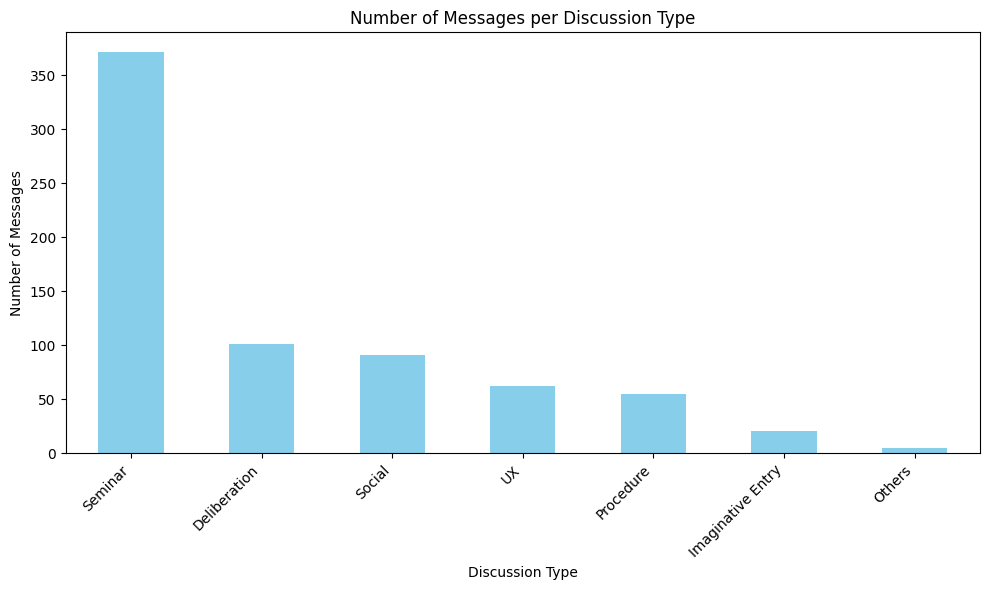
\includegraphics[width=\linewidth]{report/fig/classes distribution.png}
        \caption{Classes distribution}
        \label{fig:classes_distribution}
\end{figure}

\begin{figure}[ht]\centering
	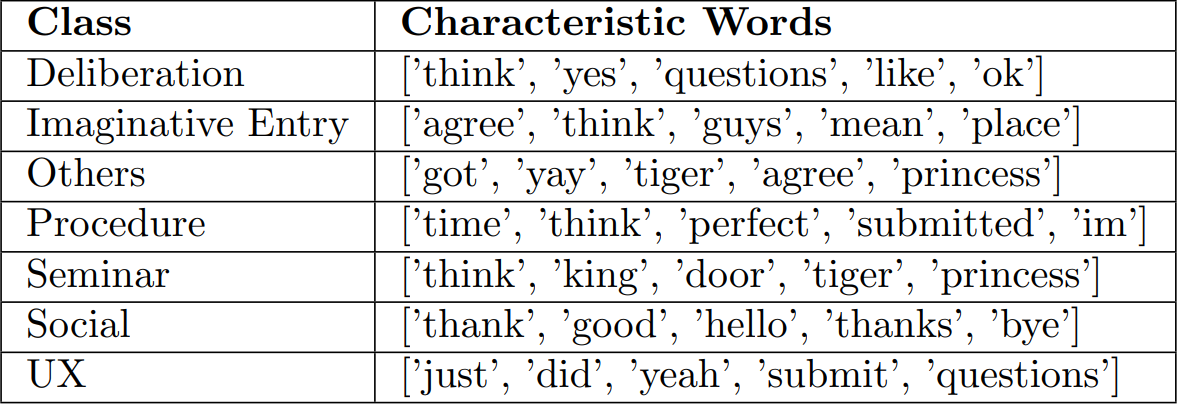
\includegraphics[width=\linewidth]{report/fig/tabela_besed.png}
        \caption{Most Characteristic Words for Each Class}
        \label{fig:words_class}
\end{figure}




\subsection*{Implementation with analysis}

In this section we will look at text categorization task that was solved with tf-idf and bag-of-words representation which we used to train different machine learning models. After preprocessing all available data we used messages from different forums and their human annotated labels. Every message was converted to vector depending on chosen representation and forwarded to machine learning models with associated label. The models we used are XGBoost, Logistic Regression, Random Forest, and SVM. In table \ref{tab:results} we can see the results for every technique under section Results. For evaluation we used 5-fold cross validation where we computed F1 score with micro averaging. From results we can observe that there is not one universal ML model that will perform best on different representation so it is important to fine tune the classificator in our LLM implementation.


\subsection*{Implementation with base BERT}

We started this implementation the same way we started in the previous section by importing the preprocessed data. The first task was preparing the data to be accepted by the BERT model. First we made mappings for converstion from labels to ids, which are used by the model. Afterwards we tokenized the messages to the vocabulary that the model uses. This was accomplished using datasets and a Bert Tokenizer. We also split the data into the train (70\%), validation (15\%) and test (15\%) set. For the first test we used a model for sequence classification using the bert model (more specifically the bert base cased). As in the previous tasks we decided to look at the f1 micro score, but we also added a confusion matrix for the results to better understand the model. For the training part we decided to run the learning proces for 10 epochs. \cite{bert} \cite{bertHF}

\subsection*{Implementation with large BERT on HPC}

As we wanted to improve the results gotten by the base bert model in the previous subsection, we also trained another Bert For Sequence Classification that is based on the large bert model. As the training time on our gpu was starting to get quite long, we decided to train the model on the Arnes HPC. While the environment setup with SLURM took a long time it was worth it in the end as the training time was reduced by a lot using only one node with the Nvidia V100 gpu. The setup was the same as in the previous sub section with the same sized train, test and validation splits (70/15/15). For training we decided to run for 10 epochs as we didnt see much improvments afterwards. \cite{sling}

\subsection*{Using ChatGPT to categorize text}
Another technique we used is prompting capable pretrained LLMs. The best results were achieved with gpt3.5-turbo model but we didn't try gpt4 model. The main idea was to use LLMs knowledge of text categorization with provided definitions for each category. We tried zero-shot and few-shot and found out that few-shot prompting drastically improved performance measured with F1-micro score.


\begin{figure}[ht]\centering
	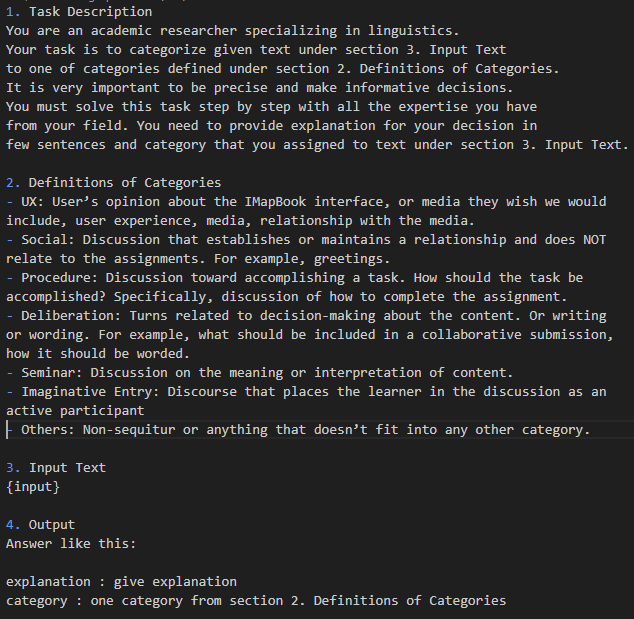
\includegraphics[width=\linewidth]{report/fig/zero-shot-prompt.png}
        \caption{Ours zero shot prompt with definitions.}
        \label{fig:zeroshot}
\end{figure}

\begin{figure}[ht]\centering
	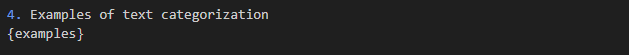
\includegraphics[width=\linewidth]{report/fig/monkeybusiness.png}
        \caption{Addition for few-shot prompting.}
        \label{fig:fewshot}
\end{figure}

In figure \ref{fig:zeroshot} we can see the prompt with definition for each category. On top we added task description and assigned a persona to GPT model. We also included input text section where we dynamically changed text that needed categorization and at the end specified in what format output must be returned. As you can see from the figure we also added explanation output which is interesting to see why model decided for specific category.

In figure \ref{fig:fewshot} we can observe that we added another section where we dynamically included text samples and their categories which were then excluded from evaluation set. This technique was the reason for much better categorization performance. Here are the number of text samples that were included randomly for every category: "UX": 2, "Social": 2, "Procedure": 2, "Deliberation": 3, "Seminar": 5, "Imaginative Entry": 3, "Others": 2. These numbers were picked intuitively and there is room for optimization. The results for both techniques are stated under section Results in table \ref{tab:results}.


\section*{Results}

\begin{table}[h]
\centering
\caption{Results of different ML models using tf-idf representation.}
\vspace{0.3cm}
\label{tab:results}
\begin{tabular}{|c|c|c|c|c|}
\hline
TF-IDF & XGB & LR & RF & SVM \\
\hline
F1-micro & 0.5927 & 0.6095 & 0.5492 & 0.6025 \\
\hline
BoW & XGB & LR & RF & SVM \\
\hline
F1-micro & 0.6062 & 0.5878 & 0.5666 & 0.6246 \\
\hline
BERT & Base (val) & test & Large (val) & test  \\
\hline
F1-micro & 0.733 & 0.726 & 0.75 & 0.698 \\
\hline
GPT3.5 & Zero & / & Few & / \\
\hline
F1-micro & 0.2719 & / & 0.6360 & / \\
\hline
\end{tabular}
\end{table}

\subsection*{Base BERT}
After training the neural model we got an f1 micro score on the validation set of 0.733 and on the test set we got an f1 micro score of 0.726. Below in Figure 5 we can see the confusion matrix for the test set for a better analysis of the results. 

\begin{figure}[ht]\centering
	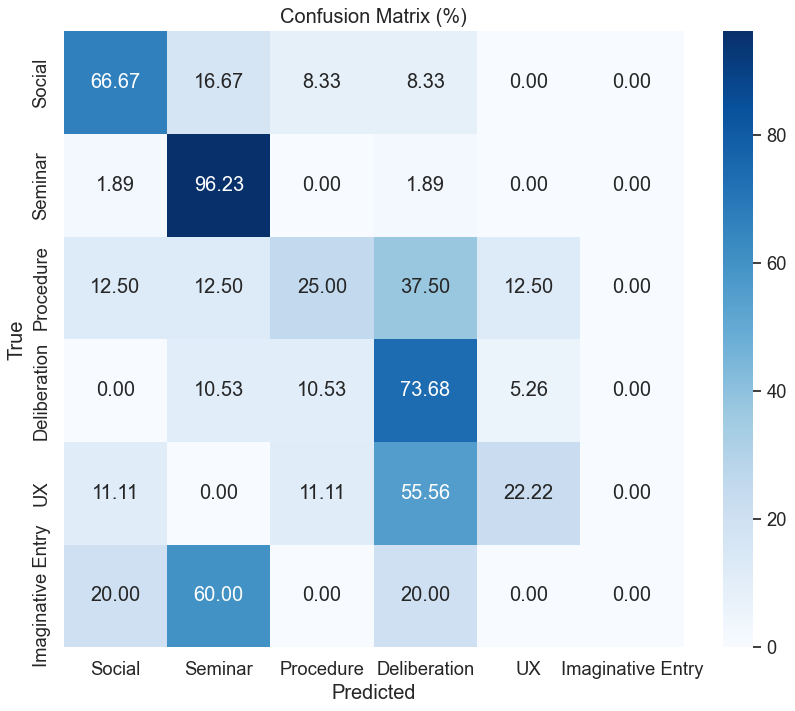
\includegraphics[width=\linewidth]{report/fig/image.png}
    \caption{Confusion matrix for base bert test results}
	\label{fig:column}
\end{figure}

\subsection*{Large BERT on HPC}
 Regarding the results of the large bert model, we expected a slight improvment compared to the base model. However we were underwhelmed by the results as they were very similar to the base model. After training the neural model on the HPC we got an f1 micro score of 0.75 on the validation set and an f1 micro score of 0.698 on the test set. In Figure 6 we can also see the confusion matrix for the test set. If we compare it with the base BERT model, we can see there are some improvments on certain classes, but also some worse results for others. Interestingly both of the models completly failed the Imaginative Entry class predictions, howerver it is important to note that because this class is underrepresented and consequently there are only 5 examples in the test set, we can excpect that the results for this class would be worse and unstable.

\begin{figure}[ht]\centering
	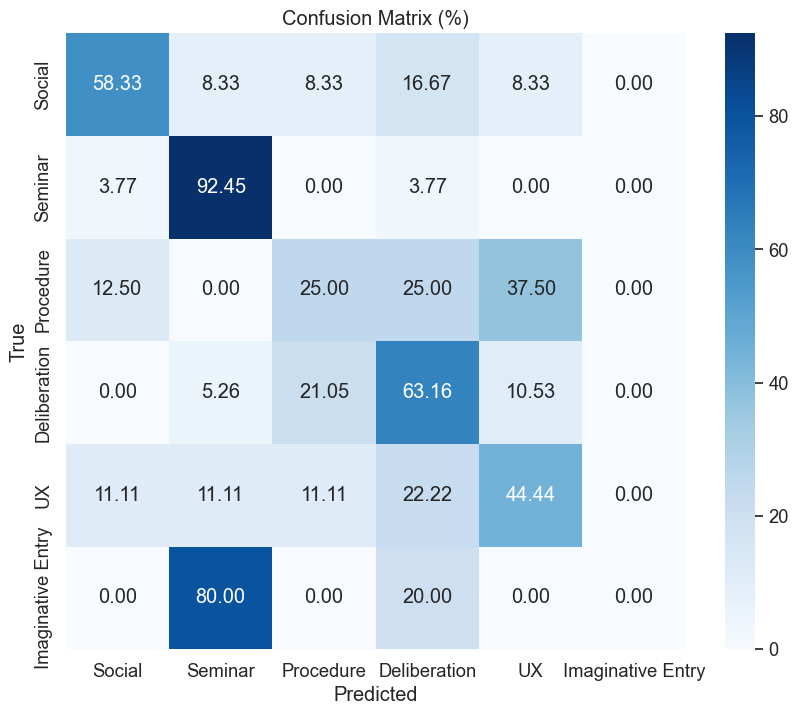
\includegraphics[width=\linewidth]{report/fig/confusion_matrix_HPC.png}
    \caption{Confusion matrix for large bert test results}
	\label{fig:column}
\end{figure}

\subsection*{GPT-3.5 Categorization Explanations}
We also asked ChatGPT 3.5 to explain its classifications of the following dialogue examples. Chat classified "Hello" as a Social type with the explanation that "Hello" is a typical greeting used to initiate a conversation or establish a social connection. It does not relate to any specific task, decision-making, interpretation of content, or user experience. This classification was deemed correct.

Next, we examined the following example: "The emphasis on barbarism implies that she sent him to the lion." Chat classified this dialogue as Seminar type and explained that the text discusses the implication of emphasizing barbarism concerning a female character sending someone to face a lion. It involves interpreting the meaning behind the actions of the character. This classification was also deemed correct.

Last, we examined "I agree with Cassandra's noticing." Chat classified this dialogue as Social type, asserting that the text indicates a response to someone named Cassandra, expressing agreement with something she observed or pointed out. This text does not involve establishing a relationship, discussing a task procedure, decision-making, interpreting content, imaginative entry, or being a non-sequitur. However, this classification was incorrect, as it actually belonged to the Seminar type.
9


\section*{Conclusion}

%Use the Discussion section to objectively evaluate your work, do not just put praise on everything you did, be critical and exposes flaws and weaknesses of your solution. You can also explain what you would do differently if you would be able to start again and what upgrades could be done on the project in the future.

This study explored using large language models (LLMs) to automate qualitative discourse analysis of online discussions, focusing on "The Lady, or the Tiger?" Initially, traditional methods like TF-IDF and bag-of-words were used to train various classifiers, achieving moderate success. Advanced models like BERT were then employed, significantly improving accuracy (validation accuracy of 0.733 and test accuracy of 0.726). Additionally, GPT-3.5 was used with zero-shot and few-shot prompting, with few-shot prompting notably enhancing performance (F1-micro score of 0.636). Our goal was demonstrating that advanced LLMs, especially when fine-tuned and properly prompted, can effectively have decent performance in discourse analysis. There is still room for future research in automating complex qualitative tasks using LLMs especially with larger datasets.
%------------------------------------------------



%----------------------------------------------------------------------------------------
%	REFERENCE LIST
%----------------------------------------------------------------------------------------
\bibliographystyle{unsrt}
\bibliography{report}


\end{document}